\chapter{نمایش نتایج نمونه}
اعداد این فصل ساختگی‌اند و تنها برای آموزش درج نمودار آمده‌اند.
\section{نمودار}
\begin{ThesisChart}
\centering
% Synthetic demonstration values only; heights are in centimetres.
\def\SampleA{2}\def\SampleB{3}\def\SampleC{4}

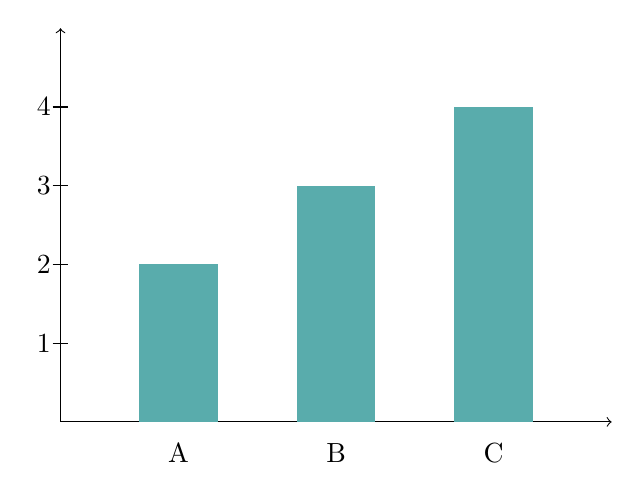
\begin{tikzpicture}
\draw[->] (0,0)--(7,0);\draw[->] (0,0)--(0,5);
\fill[teal!65] (1,0) rectangle (2,\SampleA);
\fill[teal!65] (3,0) rectangle (4,\SampleB);
\fill[teal!65] (5,0) rectangle (6,\SampleC);
\node at (1.5,-.4) {\lr{A}};\node at (3.5,-.4) {\lr{B}};\node at (5.5,-.4) {\lr{C}};
\foreach \y in {1,2,3,4} {\draw (-.1,\y)--(.1,\y);\node[left] at (0,\y) {\lr{\y}};}
\end{tikzpicture}

\caption[مقایسه ساختگی]{مقایسه سه مقدار ساختگی از پوشه داده‌های نمونه؛ از این نمودار نباید نتیجه پژوهشی گرفت.}\label{fig:chart}
\end{ThesisChart}
مقادیر از یک پرونده مشترک خوانده می‌شوند؛ با تغییر داده‌ها و ساخت دوباره، نمودار به‌روز می‌شود.
